\newcommand{\tensor}[1]{\mathcal{#1}}
\newcommand{\tens}[1]{\tensor{#1}}

\newcommand{\vect}[1]{\textbf{#1}}

\newcommand{\naam}[1]{\textit{#1}}

\newcommand{\R}{\mathbb{R}}
\newcommand{\N}{\mathbb{N}}
\newcommand{\I}{\mathbb{I}}
\newcommand{\ii}{\vect{i}}




\documentclass[11pt]{IEEEtran}

\usepackage{amsfonts, amsmath}
\usepackage[english]{babel}

\usepackage{graphicx}

\title{Parallelisation of calculations with matrices using OpenCL}
\author{Daan Wendelen}

\begin{document}
\maketitle

\section{Tensors}
We can represent a tensor as a $N$-dimensional array. A $N$-dimensional tensor is called a $N$-th order tensor. A $N$-th order tensor has $N$ modes. A tensor in defined as:
\[
	\tensor{T} \in \R^{I_1 \times \dotsb \times I_N}
\]
We also define the collection of all valid indices of a tensor as:
\[
    \I = \{\ii{} \in \N_0^N | \forall n \in [1, N]: i_n \in [1, I_n]\}
\]

Tensors can be decomposed. One of those decompositions is the Canonical Polyadic Decomposition (CPD). The elements of \TT{} can be calculates in the following manner: 
\[
    t_{\ii{}} \approx c_{\ii{}} = \sum_{r=1}^{R} \prod_{n=1}^{N} u^{(n)}_{i_{n}r}
\]
\centering{with $\ii{} \in \I$, $R \in \N_0$ and $\mUU{n} \in \R^{I_n \times R} $}

The CPD \CC{} is an approximation of \TT{}. We therefor define the residu tensor as:
\[
    \F = \C - \T
\]
We define the goal function $f(\T, \mUUU)$ as the frobenius norm of \FF{}.
\[
    f(\T, \mUUU) = \sum_{\ii{} \in \I} \left( \left( \sum_{r=1}^{R} \prod_{n=1}^{N} u^{(n)}_{i_{n}r} \right) - t_{\ii{}} \right)^2
\]
The goal of many algorithms is to find the factormatrices \UUU{} for which $f$ is the smallest. One group of such algorithms are the gradient based optimization algorithms. They have in common that they use the gradient of $f$ to find the best approximation of \TT. The gradient can be calculated with the following formula.
\[
    g^{(n)}_{ir} :=\sum_{\substack{\iii{} \in \I\\ i'_n = i}} f_{\iii{}} \prod_{\substack{n'=1\\n'\neq n}}^{N} u^{(n')}_{i'_{n'}r}
\]
We call \GGG{} the gradientmatrices.

\section{OpenCL}
OpenCL is a framework for parallel computation. We can use OpenCL on both CPU's and on GPU's. We will focus on the GPU.

A GPU consist of a number of compute-units. Every compute-unit can run 64 threads in parallel. These 64 threads always execute
the same instruction at the same time. This means that one thread can stall the whole compute unit. A set of 64 threads is called a wavefront. And a compute unit can switch between wavefronts. A wavefront always runs on the same compute unit.

The GPU also has memory. The memory is served by several channels. When multiple compute-units try to access the same channel, at the same time, a channel conflict occurs. When this happens, one of the compute units stalls. A compute unit can access multiple channels at the same time. When we request data from the memory it takes 300 to 600 cycles to arrive. This is called the latency of the memory. It is important to have enough threads active to occupy the compute unit while another thread is waiting for the data to arrive.

\section{Kernels for calculating f(T, U)}
We focus on thirth order tensors that wil be calculated on the AMD Radeon HD 6970.

\subsection{Is it suitable for parallelisation?}
Before we develop a kernel, we first do some research to validate that the algorithm is suitable to run in parallel on the graphics card. We validate that the algorithm is able to use all the computational power of the GPU. Some algorithms are not suitable because they are bound by the bandwidth. For other algorithms it is simply not possible to parallelise them.

We call the ratio between the number of flop's and the amount of memory transactions, the computation ratio. A high ratio is preferred because it means we can utilise more computational power. (if it is available) A low ratio indicates that the memory will be the bottleneck.

Our research indicated that $f$ is suitable for parallelisation when $I > 40$ and $R > 15$ for calculations in double precision. In single precision $I$ must be greater than 40 and $R$ must be greater than 31.

\subsection{The kernels}
 We developed several kernels. The first one the float8x8x8. With the float8x8x8, every wavefront is assigned a $8 \times 8 \times 8$ block of the tensor. This is about just enough to balance the speed of the compute unit, with the speed of the memorf. A variant on this kernel is the float16x16x16. With this kernel every wavefront is assigned a $16 \times 16 \times 16$ block of the tensor. As the name suggested. The float16x16x16 has a much better computation ratio.
 
 The problem with these kernels is that all wavefronts access multiple channels of the memory. This leads to channel conflicts and channel conflicts lead to a drop in performance. To tackle this issue, we also developed a few kernel which suffer less from this phenomenon. The strategy is to relocate the elements of \TT{} to locations that cause fewer channel conflicts.   The new kernels are called float16x16x16R (Remapped), float16x16x16I (Isolated) and float8x8x8R.

 
\section{Kernels for calculating \GGG{}}
\subsection{Modifying double16x16x16}
We need to use \FF{} to calculate the gradient. We can get \FF{} as a side effect of calculating $f$. We therefor need to modify for example double16x16x16 to write \FF{} to the buffer. The modified version is called double16x16x16FG. Note we use doubles. All algorithms can be modified to use double's instead of float's. This modification halfs the computation ratio. double16x16x16FG is suitable for parallelisation when $I > 40$ and $R > 30$ for calculations in double precision. In single precision $I$ must be greater than 40 and $R$ must be greater than 62.

\subsection{Is it suitable for parallelisation?}
We also need to verified that calculation of the gradient is suitable for parallelisation. The computation ratio of for computing the gradient is about the same as the ratio for computing $F$. We conclude that the gradient is suitable for parallelisation when $I > 40$ and $R > 15$ for calculations in double precision. In single precision $I$ must be greater than 40 and $R$ must be greater than 31.

\subsection{double16x16G}
The kernel that calculates the gradient is called double16x16G. We gave it that name because a wavefront is assigned to a $16 \times 16$ block of the gradientmatrix. We also had to create a new kernel to calculate f(\TT, \UUU) which writes \FF{} to the memory as a side effect. We call this 

\section{Results}
We executed all kernels for different values for $R$ en $I$ and measured the time it took the kernel to complete its execution. This time does not include the time necessary to transfer data from and to the memory. The time is measured using the profiling information provided by the OpenCL API and it has a resolution of 1 ns. \cite[p.~4-13]{amd} We use this time to measure the computational power that the implementatie achieves. \cite[p.~4-13]{amd}

\subsection{Kernels for calculating f(\TT, \UUU)}
In all the following plots we increase $I$ from 16 to 320 in steps of 16 with $R=8, 16, 400, 4000$

\subsubsection{Float16x16x16 and float8x8x8}
\begin{figure}[h]
\centering
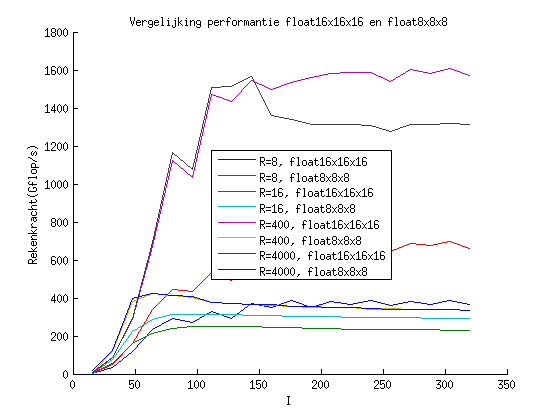
\includegraphics[width=0.5\textwidth]{fl16_vs_fl8_groot}
\caption{\label{fl16_vs_fl8} Comparing the performance of float16x16x16 and float8x8x8 for different value of $R$ and $I$.}
\end{figure}

For $I$ = 16, 32, 48 we see a strong increase in performance when $I$ increases. We explain this as follows for float16x16x16. When $I$ equals 16 we only use one compute unit, when $I$ equals 32 we use eight of them and when $I$ equals 48 we use all compute units. For float8x8x8 we use eight compute units when $I$ equals 16 and we use all compute units when $I$ exceeds 32.

Even after all compute units are used we can still see an increase in performance when $I$ increases. This is because the compute unit starts executing other work groups when the current work group is waiting for data from the memory.

After that the performance is somewhat contant with one exception. For float16x16x16 for $R=4000$ at $I=144$ we see a decrease of performance. We believe that there are just to many cache misses to keep compute units going.

The highest value we measured is 1610 Gflop/s. This is almost 60\% of the theoretical maximal computational power of our graphics card. We reach this value with float16x16x16 with $R=400$ and $I=304$. The other 40\% is lost by switching work-groups on the compute unit, redundant calculations and bookkeeping like calculating indices.


\subsubsection{Float16x16x16 and float16x16x16R}
\begin{figure}[h!]
\centering
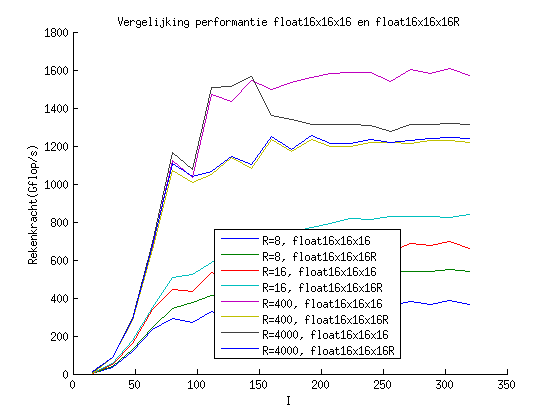
\includegraphics[width=0.5\textwidth]{fl16_vs_fl16R}
\caption{\label{fl16_vs_fl16R} Comparing the performance of float16x16x16 and float16x16x16R for different value of $R$ and $I$.}
\end{figure}

Float16x16x16R heeft als doel om het aantal geheugen conflicten te beperken. We willen graag zien of dit effectief gelukt is. Zie figuur \ref{fl16_vs_fl16R} voor een vergelijking van de performatie. We moeten een onderscheid maken tussen twee situaties. $R$ in de groeifase en $R$ in de constante fase.

Voor $R$ in de groeifase zien we dat float16x16x16R het duidelijk beter doet dan float16x16x16 wanneer $I$ wat groter is. Dit komt omdat in de groeifase de rekenkracht beperkt wordt door de bandbreedte. Door het aantal kanaalconflicten te verlagen kunnen we veel beter gebruik maken van die bandbreedte.

Wanneer $R$ in de constante fase is zijn de rollen omgekeerd. Na $I=96$ blijft de performantie van float16x16x16 verder groeien terwijl de performantie van float16x16x16R niet meer groeit.

Wanneer $I$ klein is zien we in alle gevallen dat float16x16x16 en float16x16x16R nagenoeg samenvallen. Dit komt omdat de kanaalconflicten dan nog niet het knelpunt is en dus slechts een beperkte, maar wel zichtbare, invloed hebben op de performantie.



%\subsection{Vergelijking tussen float16x16x16R en float16x16x16I}
\begin{figure}[h!]
\centering
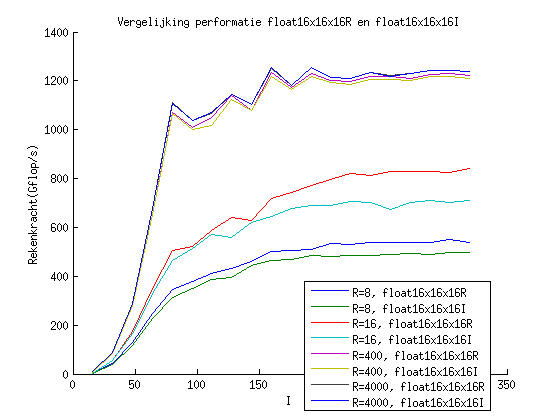
\includegraphics[width=0.5\textwidth]{fl16R_vs_fl16I}
\caption{Comparing the performance of float16x16x16R and float16x16x16I for different value of $R$ and $I$.}
\end{figure}

Float16x16x16R en float16x16x16I zijn beiden kernels die als doel hebben om het aantal geheugen conflicten te beperken. Zie figuur \ref{fl16R_vs_fl16I} voor een vergelijking van de performatie. We zien duidelijk dat float16x16x16R het overal beter doet dan float16x16x16I. Daarom gaan we verder geen aandacht meer besteden aan float16x16x16I.

%\subsection{Vergelijking tussen float16x16x16 en float8x8x8}

\begin{figure}[h!]
\centering
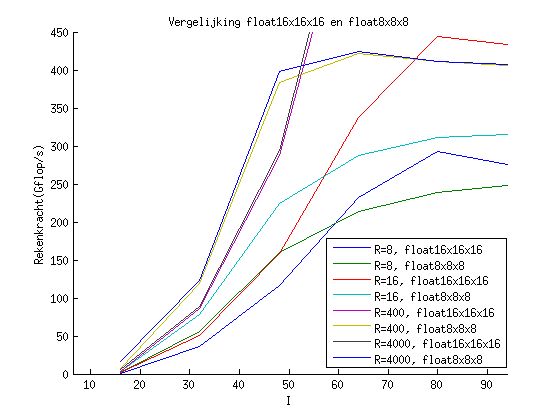
\includegraphics[width=0.5\textwidth]{fl16_vs_fl8_klein}
\caption{\label{fl16_vs_fl8_klein} Comparing the performance of float16x16x16 and float8x8x8 for different value of $R$ and $I$.}
\end{figure}

Zie figuur \ref{fl16_vs_fl8} voor een vergelijking tussen float16x16x16 en float8x8x8. Voor $I$ groter dan 64 zien we dat float16x16x16 veel beter presteert dan float8x8x8. Dit komt omdat float16x16x16 veel minder redundante berekeningen en geheugenoperaties moet doen dan float8x8x8. (Zie \ref{h:fl8_rekenverhouding} onder het punt 'Rekenverhouding')

Maar float8x8x8 heeft ook een voordelen. Omdat een work-group maar 8$\times$8$\times$8 groot is, zijn er meer work-groups nodig voor dezelfde hoeveelheid elementen. Waardoor de CU's beter benut worden. Zie figuur \ref{fl16_vs_fl8_klein} voor een beter zicht hierop. We zien dat float8x8x8 beter presteert dan float16x16x16 wanneer $I$ nog klein is. Het is pas later dat float16x16x16 de bovenhand haalt.

%\subsection{Vergelijking tussen float8x8x8 en float8x8x8R}

\begin{figure}[h!]
\centering
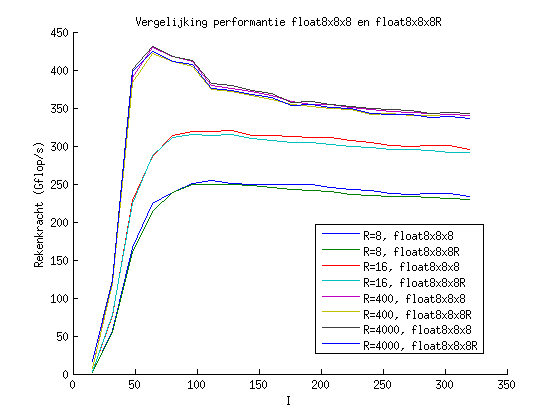
\includegraphics[width=0.5\textwidth]{fl8_vs_fl8R}
\caption{\label{fl8_vs_fl8R} Comparing the performance of float8x8x8 and float8x8x8R for different value of $R$ and $I$.}
\end{figure}

Zie figuur \ref{fl8_vs_fl8R} voor een vergelijking tussen float8x8x8 en float8x8x8R. We zien dat float8x8x8 het er overal een heel klein beetje beter doet dan float8x8x8R. We kunnen dus beter geen aandacht besteden aan float8x8x8R.

%\section{Kernels die \GGG{} berekenen}
\begin{figure}[h!]
\centering
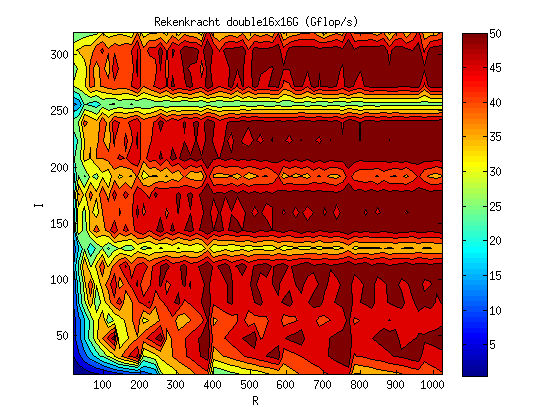
\includegraphics[width=0.5\textwidth]{result_gradient}
\caption{\label{result_gradient} Computational power of double16x16G in function of $R$ and $I$}
\end{figure}

Zie figuur \ref{result_gradient} voor de rekenkracht van double16x16G in functie van $R$ en $I$. We hebben $I$ laten oplopen van 16 tot en met 320 in stappen van 16, en $R$ van 16 tot en met 1024 in stappen van 16.

Wat meteen opvalt is dat de performantie sterk daalt wanneer $I$ een veelvoud is van 64. We kunnen dit niet verklaren maar we vermoeden dat het veroorzaakt kan worden door de ligging van de elementen in het geheugen.

Wanneer we naar de waardes van de rekenkracht kijken zien we dat we niet meer dan 54 Gflop/s halen in dubbele precisie. Dit is amper 8\% van de capaciteit van de grafische kaart.

\section{Conclusion}

\bibliographystyle{abbrv}
\bibliography{referenties}

\end{document} 

